\documentclass[tikz,border=16pt]{standalone}

\usepackage[T1]{fontenc}
\usepackage[utf8]{inputenc}
\usepackage{amsmath,amssymb}
\usetikzlibrary{shapes.geometric, arrows.meta, positioning, calc, fit, backgrounds}

% Modern color palette
\definecolor{slateborder}{RGB}{148, 163, 184}
\definecolor{slatebg}{RGB}{248, 250, 252}
\definecolor{slatetext}{RGB}{30, 41, 59}

\definecolor{blueborder}{RGB}{37, 99, 235}
\definecolor{bluebg}{RGB}{239, 246, 255}
\definecolor{bluetext}{RGB}{30, 58, 138}

\definecolor{amberborder}{RGB}{217, 119, 6}
\definecolor{amberbg}{RGB}{254, 243, 199}
\definecolor{ambertext}{RGB}{146, 64, 14}

\definecolor{greenborder}{RGB}{22, 163, 74}
\definecolor{greenbg}{RGB}{240, 253, 244}
\definecolor{greentext}{RGB}{20, 83, 45}

\definecolor{purpleborder}{RGB}{147, 51, 234}
\definecolor{purplebg}{RGB}{250, 245, 255}
\definecolor{purpletext}{RGB}{88, 28, 135}

\definecolor{tealborder}{RGB}{13, 148, 136}
\definecolor{tealbg}{RGB}{240, 253, 250}
\definecolor{tealtext}{RGB}{19, 78, 74}

\definecolor{darkblue}{RGB}{29, 78, 216}

\begin{document}
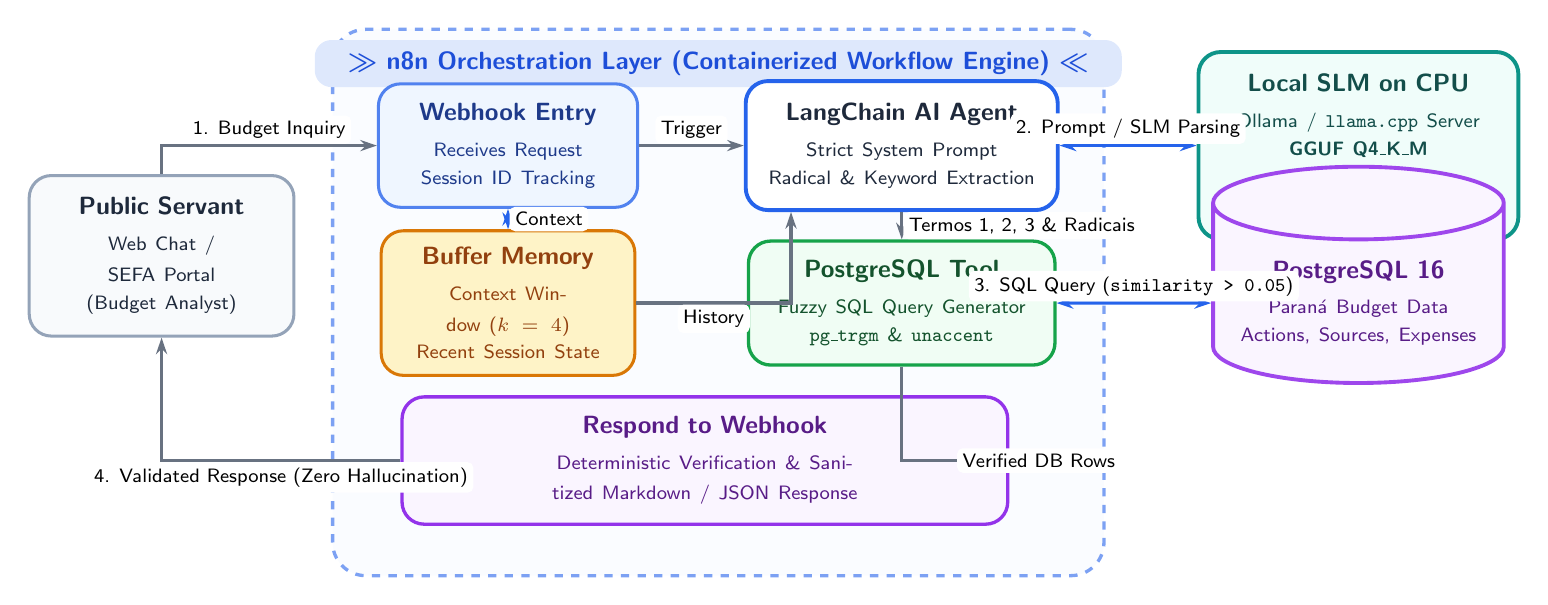
\begin{tikzpicture}[
    font=\sffamily\small,
    userbox/.style={
        rectangle, rounded corners=8pt,
        draw=slateborder, fill=slatebg, line width=1.1pt,
        inner sep=8pt, align=center, text width=2.8cm, minimum height=1.4cm,
        text=slatetext
    },
    box/.style={
        rectangle, rounded corners=8pt,
        draw=blueborder!80, fill=bluebg, line width=1.1pt,
        inner sep=7pt, align=center, text width=2.8cm, minimum height=1.2cm,
        text=bluetext
    },
    agentbox/.style={
        rectangle, rounded corners=8pt,
        draw=blueborder, fill=white, line width=1.4pt,
        inner sep=8pt, align=center, text width=3.4cm, minimum height=1.5cm,
        text=slatetext
    },
    memorybox/.style={
        rectangle, rounded corners=8pt,
        draw=amberborder, fill=amberbg, line width=1.1pt,
        inner sep=6pt, align=center, text width=2.8cm, minimum height=1.1cm,
        text=ambertext
    },
    toolbox/.style={
        rectangle, rounded corners=8pt,
        draw=greenborder, fill=greenbg, line width=1.2pt,
        inner sep=7pt, align=center, text width=3.4cm, minimum height=1.2cm,
        text=greentext
    },
    respbox/.style={
        rectangle, rounded corners=8pt,
        draw=purpleborder, fill=purplebg, line width=1.2pt,
        inner sep=7pt, align=center, text width=7.2cm, minimum height=1.1cm,
        text=purpletext
    },
    slmbox/.style={
        rectangle, rounded corners=8pt,
        draw=tealborder, fill=tealbg, line width=1.4pt,
        inner sep=8pt, align=center, text width=3.5cm, minimum height=1.6cm,
        text=tealtext
    },
    dbbox/.style={
        cylinder, shape border rotate=90, aspect=0.25,
        draw=purpleborder!90, fill=purplebg, line width=1.4pt,
        inner sep=7pt, align=center, text width=3.2cm, minimum height=1.6cm,
        text=purpletext
    },
    arrow/.style={
        -{Stealth[length=6pt, width=4pt]},
        line width=1.2pt, draw=slateborder!70!black
    },
    darrow/.style={
        {Stealth[length=6pt, width=4pt]}-{Stealth[length=6pt, width=4pt]},
        line width=1.2pt, draw=blueborder
    },
    lbl/.style={
        fill=white, inner sep=2pt, font=\sffamily\scriptsize, rounded corners=2pt
    }
]

% 1. Usuario (Client)
\node[userbox] (user) at (0, 2.0) {
    \textbf{Public Servant}\\[2pt]
    {\scriptsize Web Chat / SEFA Portal}\\[-1pt]
    {\scriptsize (Budget Analyst)}
};

% 2. Camada n8n
\node[box] (entry) at (4.4, 3.4) {
    \textbf{Webhook Entry}\\[2pt]
    {\scriptsize Receives Request}\\[-1pt]
    {\scriptsize Session ID Tracking}
};

\node[memorybox] (memory) at (4.4, 1.4) {
    \textbf{Buffer Memory}\\[2pt]
    {\scriptsize Context Window ($k=4$)}\\[-1pt]
    {\scriptsize Recent Session State}
};

\node[agentbox] (agent) at (9.4, 3.4) {
    \textbf{LangChain AI Agent}\\[2pt]
    {\scriptsize Strict System Prompt}\\[-1pt]
    {\scriptsize Radical \& Keyword Extraction}
};

\node[toolbox] (tool) at (9.4, 1.4) {
    \textbf{PostgreSQL Tool}\\[2pt]
    {\scriptsize Fuzzy SQL Query Generator}\\[-1pt]
    {\scriptsize \texttt{pg\_trgm} \& \texttt{unaccent}}
};

\node[respbox] (resp) at (6.9, -0.6) {
    \textbf{Respond to Webhook}\\[2pt]
    {\scriptsize Deterministic Verification \& Sanitized Markdown / JSON Response}
};

% 3. Motores de IA e Banco de Dados Local
\node[slmbox] (slm) at (15.2, 3.4) {
    \textbf{Local SLM on CPU}\\[2pt]
    {\scriptsize Ollama / \texttt{llama.cpp} Server}\\[-1pt]
    {\scriptsize \textbf{GGUF Q4\_K\_M} (AVX Vectorized)}\\[-1pt]
    {\scriptsize Zero Cloud API Dependencies}
};

\node[dbbox] (db) at (15.2, 1.4) {
    \textbf{PostgreSQL 16}\\[2pt]
    {\scriptsize Paraná Budget Data}\\[-1pt]
    {\scriptsize Actions, Sources, Expenses}
};

% Container Visual n8n com Header Claro e Espaçoso
\begin{scope}[on background layer]
    % Borda externa do container n8n com folga superior para o título
    \node[
        draw=blueborder!60, fill=bluebg!30, dashed, line width=1.2pt, rounded corners=12pt,
        fit=(entry) (memory) (agent) (tool) (resp),
        inner xsep=16pt, inner ysep=18pt
    ] (n8n_box) {};

    % Barra de cabeçalho do container n8n
    \node[
        anchor=north, font=\bfseries\sffamily\small,
        fill=blueborder!15, text=darkblue, rounded corners=6pt,
        inner xsep=12pt, inner ysep=4pt
    ] at ($(n8n_box.north)+(0, -0.15)$) {
        $\boldsymbol{\gg}$ \textbf{n8n Orchestration Layer} (Containerized Workflow Engine) $\boldsymbol{\ll}$
    };
\end{scope}

% ================= Conexoes e Fluxo de Dados =================

% 1. Consulta Inicial
\draw[arrow] (user.north) |- node[lbl, above, near end]{1. Budget Inquiry} (entry.west);

% 2. Trigger para o Agente
\draw[arrow] (entry.east) -- node[lbl, above]{Trigger} (agent.west);

% 3. Contexto de Memória
\draw[darrow] (memory.north) -- node[lbl, right]{\scriptsize Context} (entry.south);
\draw[arrow] (memory.east) -| node[lbl, below, near start]{\scriptsize History} ($(agent.south west)+(0.6, 0)$);

% 4. Inferência Local de SLM
\draw[darrow] (agent.east) -- node[lbl, above]{2. Prompt / SLM Parsing} (slm.west);

% 5. Extração de Termos e Radicais para a Ferramenta SQL
\draw[arrow] (agent.south) -- node[lbl, right]{Termos 1, 2, 3 \& Radicais} (tool.north);

% 6. Execução de Query Fuzzy no Postgres
\draw[darrow] (tool.east) -- node[lbl, above]{3. SQL Query (\texttt{similarity > 0.05})} (db.west);

% 7. Retorno dos Dados para o Nó de Resposta
\draw[arrow] (tool.south) |- node[lbl, right, near end]{Verified DB Rows} (resp.east);

% 8. Resposta Final ao Usuário (Zero Alucinação)
\draw[arrow] (resp.west) -| node[lbl, below, pos=0.25]{4. Validated Response (Zero Hallucination)} (user.south);

\end{tikzpicture}
\end{document}
